\documentclass[11pt,a4paper]{article}
\usepackage[latin2]{inputenc}
\usepackage{graphicx}
\usepackage{ulem}
\usepackage{latexsym}
\usepackage{amsmath}
\usepackage{amssymb}
\usepackage{amsthm}
\usepackage{graphicx}
\usepackage{wrapfig}
\usepackage{pseudocode}
\usepackage{url}
\usepackage[backref, colorlinks=true, citecolor=red, urlcolor=blue, pdfauthor={Jyh-Ming Lien}]{hyperref}

\newcommand{\handout}[5]{
  \noindent
  \begin{center}
  \framebox{
    \vbox{
      \hbox to 5.78in { {\bf } \hfill #2 }
      \vspace{4mm}
      \hbox to 5.78in { {\Large \hfill #5  \hfill} }
      \vspace{2mm}
      \hbox to 5.78in { {\em #3 \hfill #4} }
    }
  }
  \end{center}
  \vspace*{4mm}
}

\newcommand{\lecture}[4]{\handout{#1}{#2}{#3}{#4}{#1}}

\newtheorem{theorem}{Theorem}
\newtheorem{corollary}[theorem]{Corollary}
\newtheorem{lemma}[theorem]{Lemma}
\newtheorem{observation}[theorem]{Observation}
\newtheorem{proposition}[theorem]{Proposition}
\newtheorem{definition}[theorem]{Definition}
\newtheorem{claim}[theorem]{Claim}
\newtheorem{fact}[theorem]{Fact}
\newtheorem{assumption}[theorem]{Assumption}

% 1-inch margins, from fullpage.sty by H.Partl, Version 2, Dec. 15, 1988.
\topmargin 0pt
\advance \topmargin by -\headheight
\advance \topmargin by -\headsep
\textheight 8.9in
\oddsidemargin 0pt
\evensidemargin \oddsidemargin
\marginparwidth 0.5in
\textwidth 6.5in

\parindent 0in
\parskip 1.5ex
%\renewcommand{\baselinestretch}{1.25}

\begin{document}
\lecture{Midterm Exam Report}{Fall 2017}{Tisha Kanjilal}{Advance Algorithm Programming}
\section{Summary of the two methods}

\subsection{hedcuter method}


1. input : Image 'I', number of samples 'N', configurations 'C'

2. Generate uniform random distribution of site 'S' on image greyscale
'Ig' where number of S := N

3. initialize Centroidal Voronoi diagram CVT with C

4. Compute Weighted CVT

if configuration gpu Cgpu ==true then

\ \ input: I, S

else

\ \ input: Ig, S

endif

create

4.1. for each site s in S, do:

create a new cell called "cell", with s as its site

\ \ \ \ //Lloyd's Algorithm

\ \ \ \ 4.2 Perform Lloyd Algorithm

\ \ \ \ while distance moved is not greater than displacement Cd and
iteration 'It' is less than Ci

\ \ \ \ 4.3 compute voronoi

\ \ \ \ Increase virtual resolution of image I by subpixel sp

\ \ \ \ for each cell in cell CELL, do // here CELL is a list of all
cells

\ \ \ \ get the pixel color intensity of cell point px and py from the
image I

\ \ \ \ //the intensity is an integer value from 0 to 255 representing
the pixel color of the image from 1 - black to 255 - white

\ \ \ \ endfor



\ \ \ \ //we only require distance greater than 0 therefore use 256 and
1.0f

\ \ \ \ construct a priority queue (heap) whereby the priority point p
(first) is the one with the greatest distance , if same distance then
get the one with the biggest px and py

\ \ \ \ while priority queue not empty, do

\ \ \ \ get the cell of least priority from the priority queue (shortest
distance)



\ \ \ \ if the cell has already been moved or the cell has already been
visited:

\ \ \ \ nothing to be done, so get the next element from queue

\ \ \ \ else

\ \ \ \ if px neighbors (px-1 and px+1) and py neighbors (py-1 and py+1)
are within the boundary of the image height and width and their color
intensity is darker than the current position

\ \ \ \ move the point at current site to the position of the neighbor

\ \ \ \ endif

\ \ \ \ endif

\ \ \ \ remove cell from priority queue



\ \ \ \ 4.4 compute maximum distance moved

\ \ \ \ input: list of cells CELL, Image I, Configuration C

\ \ \ \ for each cell in CELL

\ \ \ \ if Cavg, then //Cavg - average termination , so if Cavg == true
referring the provided code.

\ \ \ \ return average distance moved by all cells

\ \ \ \ else

\ \ \ \ return total distance moved by the cell

\ \ \ \ endif

\ \ \ \ //this distance is used to by the while loop if it is greater
than the one specified then break loop

\ \ \ \ go: display result



the difference between having the gpu enabled is for performance, the
gpu is effective for graphics processing because it has a huge parallel
processing architecture.



\subsection{voronoi method}


\textbf{\textit{\textsc{\textsc{1. Generate uniform random
distribution of site 'S' on image greyscale 'Ig' where number of S := N
}}}}

\textbf{\textit{\textsc{\textsc{2. Initialize points P and edges E
to be empty.}}}}

\textbf{\textit{\textsc{\textsc{3. For each site $_{site}$ in S
do:}}}}

\ \ \ \ \textbf{\textit{\textsc{\textsc{4. create new cell $_{cell
}$ with $_{site}$ as it site:}}}}

\ \ \ \ \textbf{\textit{\textsc{\textsc{5. For each existing cell c
in C where C is set of all c do:}}}}

\ \ \ \ \textbf{\textit{\textsc{\textsc{6. find the perpendicular
bisector (line that passes through the two sites s) called Pb and store
it as critical points edgelist}}}}

\textbf{\textit{\textsc{\textsc{compute voronoi}}}}

\ \ \ \ \textbf{\textit{\textsc{\textsc{7. for each edge e of cell
c, do,}}}}

\ \ \ \ \textbf{\textit{\textsc{\textsc{8. identify the connection
between the edge e and c if edge has c}}}}

\ \ \ \ \textbf{\textit{\textsc{\textsc{9. if e is near the side of
the critical point then mark it for deletion}}}}

\ \ \ \ \textbf{\textit{\textsc{\textsc{10. if e intercept the
critical point then perform clipping on e and put the point of
interception in critical points edgelist}}}}

\ \ \ \ \textbf{\textit{\textsc{\textsc{11. if the has two points,
create new edge by connecting them, then mark it and add it to the edges
E and $_{cell}$.}}}}

\ \ \ \ \textbf{\textit{\textsc{\textsc{12. add $_{cell}$ to C}}
}}

\ \ \ \ \textbf{\textit{\textsc{\textsc{13. for each side border of
rectangle, do}}}}

\ \ \ \ \textbf{\textit{\textsc{\textsc{14. create a priority queue
P to hold the critical points and add the end points of the border to
the priority queue P}}}}

\ \ \ \ \textbf{\textit{\textsc{\textsc{15. for each edge in E do,}
}}}

\ \ \ \ \textbf{\textit{\textsc{\textsc{16. test relationship
between e and border}}}}

\ \ \ \ \textbf{\textit{\textsc{\textsc{17. if e outside border then
mark the edge for deletion}}}}

\ \ \ \ \textbf{\textit{\textsc{\textsc{18. if e intersects border
then clip e to the inside of the border and store in the queue}}}}

\ \ \ \ \textbf{\textit{\textsc{\textsc{19. create new edge to
connect adjacent points in P and add the edge to E}}}}

\ \ \ \ \textbf{\textit{\textsc{\textsc{20. delete all irrelevant
edges}}}}



\ \ \ \ \textbf{\textit{\textsc{}}}

\item \textbf{\textit{\textsc{}}}

\section{Comparison of the two methods}

1. Do you get the same results by running the same program on the same
image multiple times?

No it doesn't produce the same svg if you run the same program on the
same input multiple times, probably because the each time to program
runs it generates a random distribution of points using the current time
so unless they are run at the exact same time then it wouldn't be the
same output. therefore the same program might result in different points
distribution or samples. This has been shown in the folder
build/compare1 which has the same program running on the same image but
outputting different results, it was check by using git-diff terminal to
find the svg tags that are different.



2. If you vary the number of the disks in the output images, do these
implementations produce

No they do not because the generation algorithm used in voronoi is boost
and the one used in hedcut is opencv and the algorithm for the voronoi
differs from that of the other. voronoi uses edges and point and hedcut
just moves the image based on the intensity of pixel in the image.



3. If you vary the number of the disks in the output images, is a method
faster than the other?

Yes voronoi is faster for bigger numbers of disks while hedcut is used
for smaller ones. I found this by having 5 variations of n (n being the
number of disks) of each method and then getting 5 time and finding the
average of the times for each of the methods. Everything else stays
same. The output is tabulated below. I believe the reason for this is
because for many points there is a chance that the hedcut will keep
moving a point back an forth therefore taking longer.







\begin{table}[h]
\centering
\begin{tabular}{|l|l|l|}
\hline
N of disks & Hedcuter Method (avg of 5 runs)s (rounded to 2dp) & voronoi
Method (avg of 5 runs)s \\
\hline
200 & 12.94 & 15.28 \\
\hline
500 & 11.65 & 10.27 \\
\hline
1000 & 12.57 & 8.34 \\
\hline
2000 & 13.91 & 5.94 \\
\hline
5000 & 14.86 & 4.93 \\
\hline
\end{tabular}
\end{table}




4. Does the size (number of pixels), image brightness or contrast of
image increase or decrease

Yes, for images with more pixels the hedcut takes a longer time to
finish the process. The voronoi is constant. The information is shown
below:

The average time of 5 run on the normal image resolution and a smaller
resolution. With the parameters of 4000 disks radius of and iteration of
1000 for hedcut. Image was the fairyeyes.png

\begin{table}[h]
\centering
\begin{tabular}{|l|l|}
\hline
500x756 res:72pixels, average(s)&
450x600,res:80pixels, average(s)\\
\hline
30.04 & 12.70 \\
\hline
\end{tabular}
\end{table}


Sample image below:

\begin{table}[h]
\centering
\begin{tabular}{|l|l|}
\hline
 \begin{minipage}{.3\textwidth}
      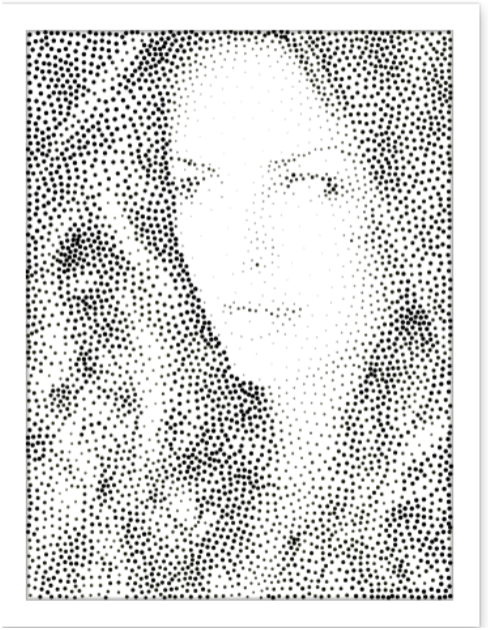
\includegraphics[width=\linewidth, height=30mm]{/Users/tishachoudhuri/desktop/media/hleft.png}
    \end{minipage}
 &
 \begin{minipage}{.3\textwidth}
      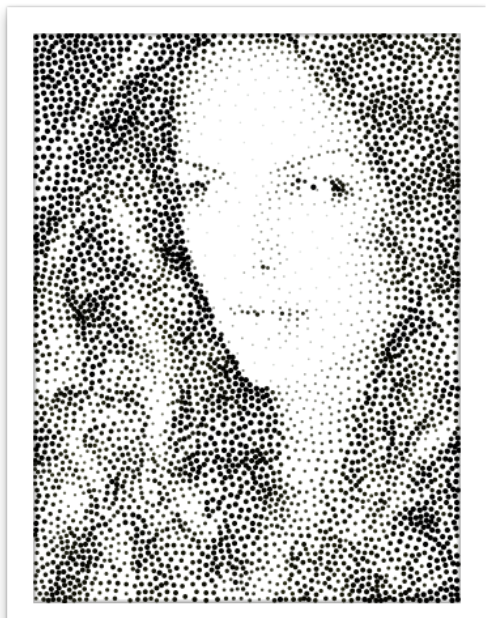
\includegraphics[width=\linewidth, height=30mm]{/Users/tishachoudhuri/desktop/media/hright.png}
    \end{minipage}
	\\
\hline
width:567pixels, height:756pixels\\
resolution:72pixels/inch (average)\\
in seconds &
width: 450pixels, height:600pixels\\
, resolution:80pixels\\
(average) in seconds \\
\hline
\end{tabular}
\end{table}




5. Does the type of image (human vs. machine, natural vs. urban
landscapes, photo vs. painting,

Yes, it does. The voronoi method performs best and output visibly
pleasing distributions, while in hedcuter method the because of the
moving of points the output is not clear, that is it does produce an
output. The size of images, the intensity of the pixels in the image and
especially color has a big effect on the hedcuter method. Below shows
the sample of hedcuter and voronoi on the klaymen.png.

\begin{table}[h]
\centering
\begin{tabular}{|l|l|}
\hline
 \begin{minipage}{.3\textwidth}
      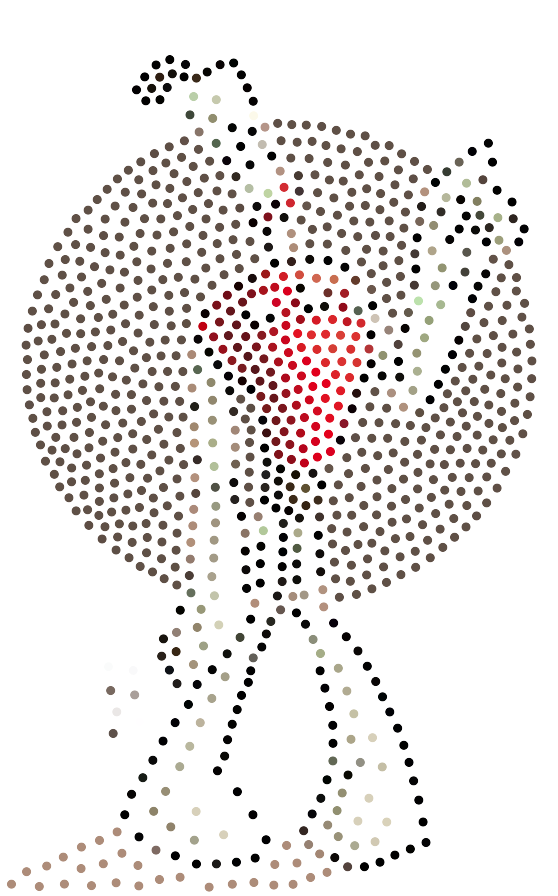
\includegraphics[width=\linewidth, height=60mm]{/Users/tishachoudhuri/desktop/media/v.png}
    \end{minipage}
 &
 \begin{minipage}{.3\textwidth}
      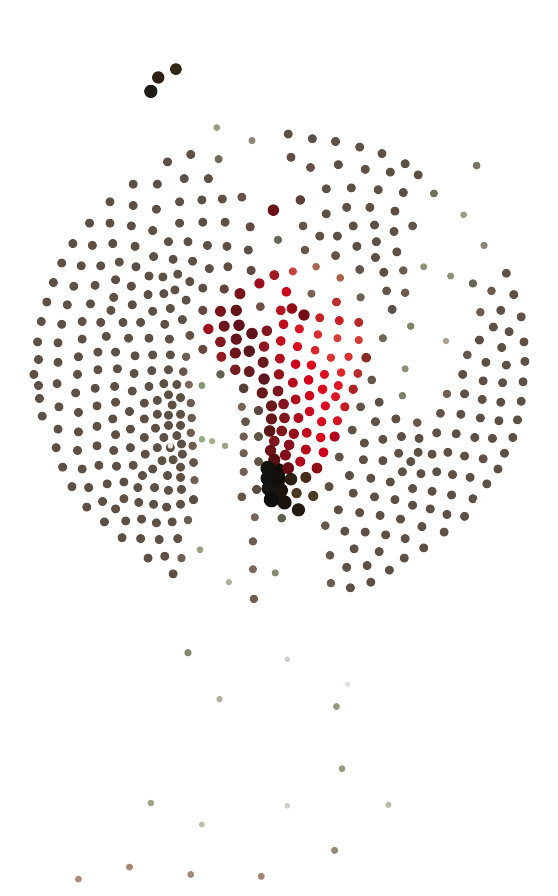
\includegraphics[width=\linewidth, height=60mm]{/Users/tishachoudhuri/desktop/media/h.png}
    \end{minipage}
  \\
\hline
voronoi Method & Hedcuter Method \\
\hline
\end{tabular}
\end{table}




6. Are the outputs of these stippling methods different the hedcut
images created by artists (e.g.

I picked up an image from wall street shown in the folder build/compare6
in the folder hedcuter/code/build. The images of the artist, voronoi
method and hedcuter method are shown below.



\begin{table}[h]
\centering
\begin{tabular}{|l|l|l|l|}
\hline
Original & Artist & voronoi Method & Hedcuter Method \\
\hline
 \begin{minipage}{.25\textwidth}
      
\includegraphics[width=\linewidth, height=30mm]{/Users/tishachoudhuri/desktop/media/orig.png}
    \end{minipage}
&
\begin{minipage}{.25\textwidth}
      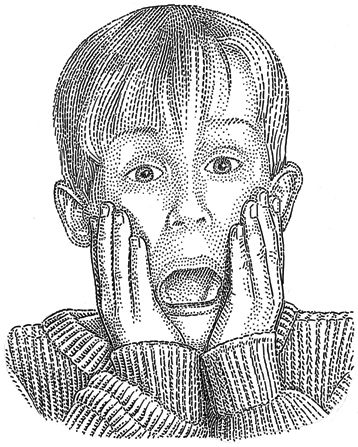
\includegraphics[width=\linewidth, height=30mm]{/Users/tishachoudhuri/desktop/media/artist.png}
    \end{minipage}
&
 \begin{minipage}{.25\textwidth}
      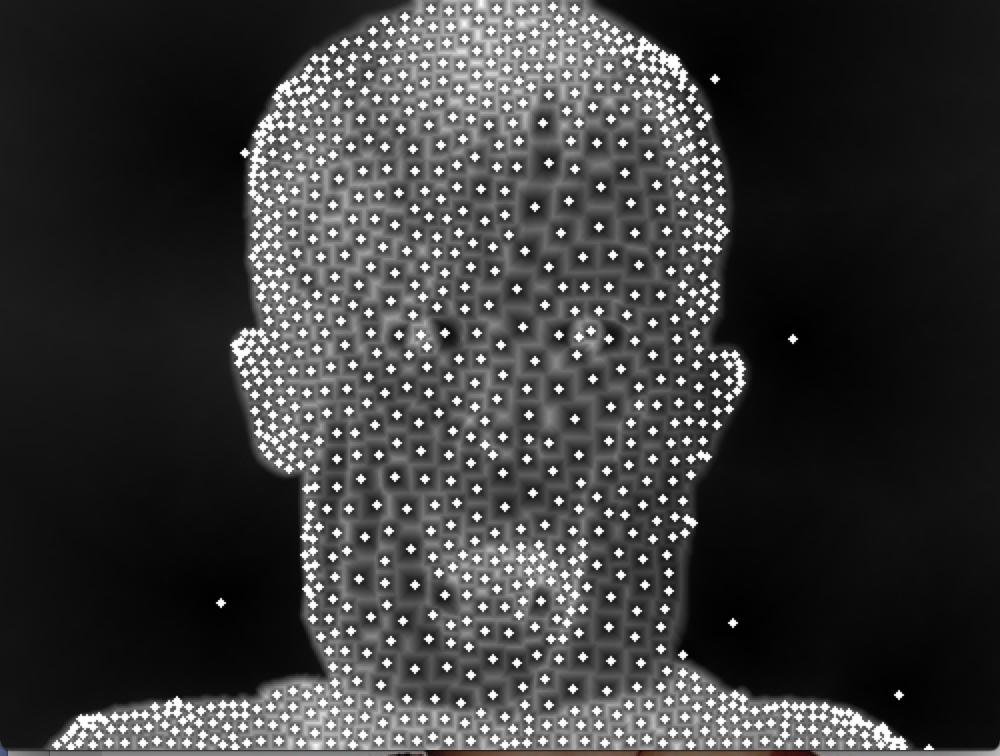
\includegraphics[width=\linewidth, height=30mm]{/Users/tishachoudhuri/desktop/media/sh.png}
    \end{minipage}
&
 \begin{minipage}{.25\textwidth}
      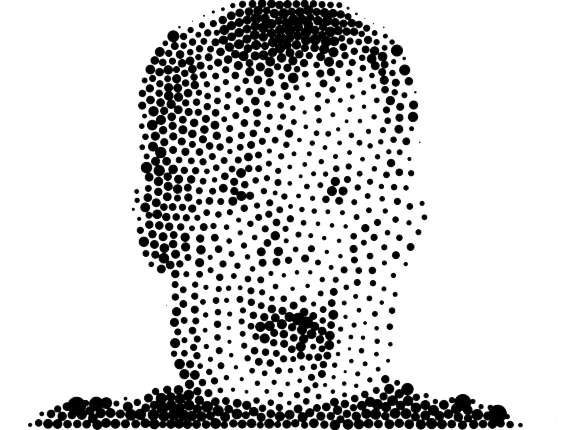
\includegraphics[width=\linewidth, height=30mm]{/Users/tishachoudhuri/desktop/media/sv.png}
    \end{minipage}\\

\end{tabular}
\\
N/A for Hedcuter Timeout two points
 kept on moving back and forth
\end{table}


It appears that the image from the artist has better tones and the radius
is much better. However in the voronoi method the image come pretty
close in the tones especially when the input from the user is limited.
The hedcuter method has a problem with colors because it works based on color intensity at a particular position in
the image and therefore in an image with high intensity it will take a lot of time moving the point from one position to another
which can go on for a very long time (performance issues).





\section{Improvement of hedcuter method}

Provide at least two improvements (each will worth 20 points) to the
hedcuter code. Below are



I added a quicker sorting algorithm using the insertion sort, that way
the number of swapping done by the std::make\_heap(open.begin(),
open.end(), compareCell); in wcvt.cpp will be less substantially
therefore reducing the time taking to compute in the hedcuter. I showed
below the time difference for the normal make heap and the one with
insertion sort of the vector before. You can do the same test by
uncommenting the start and end time in the CVT::vor(cv::Mat \& img)
method in wcvt.cpp. You can enable this by simply adding -useqsorting
(stands for use quicker sorting) to the argument when running hedcuter.

I also added a graph that will be used to uncluster the disks to improve
the distribution. You can do this by using the two options -gclusterv
(this will be in integer to specify the number of disks that are
clustered together, if the number of disks are greater than -gclusterv
then it will remove the clusters and generate another point somewhere
else) and -gclusterdist (this is the distance between disks so if the
distance between two disks is -gclusterdist it will add the edge). The
aim is that if the number of edges of a point is more than the cluster
value then uncluster.



I also wanted to add another option that will create a list for already
existing points that was if the point in hedcuter has moved to a
position it cannot move back to that position again. This will improve
the hedcuter for images with bigger resolution and also improve the
hedcuter for colored pixels. If the point is moved to that position it
will add it position to the list then everytime its going to move, it
will check the list to see if that position has been moved to already.
\bibliographystyle{plain}
\bibliography{report}
\end{document}
